\chapter{Plane-Wave Propagation}
In Chapter \ref{ch:TimeVaryingFields}, it was seen that a time-varying electric field $\vec{E}(\vec{r},t)$ produces a time-varying magnetic field $\vec{H}(\vec{r},t)$, and vice versa. Even in the absence of a source excitation, this cyclic pattern often results in an EM wave propagating through free-space or some medium. When a wave propagates in a homogenous medium without interacting with obstacles, it is said to be $\coltextit{unbounded}$. In a lossless medium (like air or a perfect dielectric), the EM wave does not get attenuated. In a lossy medium (material with a non-zero conductivity), the wave does get attenuated and some power is lost as heat. \par 

A source such as an antenna may radiate waves outwardly in the form of a \coltextit{spherical wave}. You can imagine if you drop a rock in a pond, the water waves produces travel outwardly; this is an example of a spherical wave. To an observer standing very far away from the source of a spherical wave, the spherical wave will appear as more ``flat'', as shown in Fig.\ \ref{fig:SphericalWaveFront}. 

\begin{figure}[!htp]
    \centering
    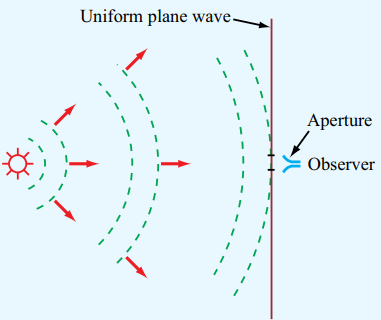
\includegraphics[width=0.3\linewidth]{images/Plane Wave Propagation/SphericalWave.png}
    \caption{Spherical-wave fronts may be approximated as a plane wave if observed at a far distance.}
    \label{fig:SphericalWaveFront}
\end{figure}

To such an observer, the spherical wave may then be approximated as a \coltextit{plane wave}. As the name suggests, a plane wave consists of a plane tangent to the direction of propagation of the wave. The plane wave has identical properties at any point on the plane (e.g. amplitude, phase, polarization, etc.). Fig.\ \ref{fig:PlaneWave} shows a visualization of a plane wave propagating through space. 

\begin{figure}[!htp]
    \centering
    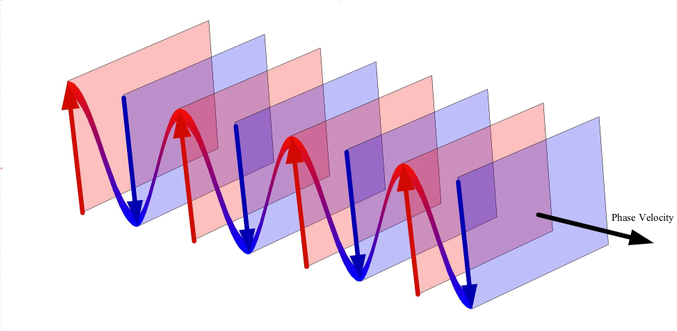
\includegraphics[width=0.5\linewidth]{images/Plane Wave Propagation/PlaneWave.png}
    \caption{Plane wave propagating in space. The red and blue planes represent when the plane wave has a maximum or minimum amplitude, respectively.}
    \label{fig:PlaneWave}
\end{figure}

Plane-waves are good approximations to real waves in many practical situations. For example, in antenna engineering, transmitting and receiving antennas are usually at such far distances from each other that the curvature of the wave fronts are negligible and plane waves may be used for analysis. \par 

When a wave propagates along a material structure, it is said to be travelling in a \coltextit{guided medium} (e.g.\ a transmission line). In Chapter \ref{ch:TransmissionLineTheory} we saw the voltage and current propagation along a transmission line. But, a transmission line can be analyzed with the propagation of electromagnetic waves as well. Thus, we may model wave propagation on a transmission line in terms of voltage and currents along its conductors, or in terms of the electric and magnetic fields in the dielectric medium between the conductors. 

% ===========================================
% Time-Harmonic Fields 
% ===========================================
\section{Time-Harmonic Fields}
Time-varying fields ($\vec{E}, \vec{D}, \vec{H}, \vec{B}$) and their sources ($\rho$, $\vec{J}$) depend on both the position in space and time $t$. But if their variation with time is sinusoidal, the fields and sources may be represented by a \textit{vector phasor} that only depends on the position $\vec{r} = (x,y,z)$. A tilde ($\sim$) will be used to denote vector phasors. For example, relationship between the time-varying field $\vec{E}$ and its corresponding vector phasor $\vecphasor{E}$ is 
\begin{equation}
    \vec{E}(\vec{r}, t) = \Re\{ \vecphasor{E}(\vec{r}) e^{j\omega t} \}
\end{equation}
Maxwell's equations for time-varying fields [Eqs.\ (\ref{eq:Maxwell1})-(\ref{eq:Maxwell4})] may be rewritten in the phasor-domain as 
\begin{align}
    \nabla \cdot \vecphasor{E} &= \dfrac{\phasor{\rho}_v}{\varepsilon} \label{eq:Maxwell_Phasor1} \\ 
    \nabla \times \vecphasor{E} &= -j\omega\mu\vecphasor{H} \label{eq:Maxwell_Phasor2} \\ 
    \nabla \cdot \vecphasor{H} &= 0 \label{eq:Maxwell_Phasor3} \\ 
    \nabla \times \vecphasor{H} &= \vecphasor{J} + j\omega\varepsilon\vecphasor{E} \label{eq:Maxwell_Phasor4}
\end{align}
By defining the \coltextit{complex permittivity} $\varepsilon_c$ as 
\begin{empheq}[box=\eqnGreenBox]{equation}
    \varepsilon_c = \varepsilon - j \dfrac{\sigma}{\omega} = \varepsilon' - j \varepsilon''
\end{empheq}
Maxwell's equations are written as 
\begin{empheq}[box=\eqnGreenBox]{align}
    \nabla \cdot \vecphasor{E} &= 0 \label{eq:Maxwell_Phasor_New1} \\ 
    \nabla \times \vecphasor{E} &= -j\omega\mu\vecphasor{H} \label{eq:Maxwell_Phasor_New2} \\ 
    \nabla \cdot \vecphasor{H} &= 0  \label{eq:Maxwell_Phasor_New3}\\ 
    \nabla \times \vecphasor{H} &= j\omega\varepsilon_c\vecphasor{E} \label{eq:Maxwell_Phasor_New4}
\end{empheq}
More about $\varepsilon_c$ is said later. See Proof \ref{proof:MaxwellEquationsPhasor} for how these were derived. \par 

The \coltextit{wave equations} for $\vecphasor{E}$ and $\vecphasor{H}$ can be shown to be 
\begin{subequations}
\begin{empheq}[box=\eqnGreenBox]{align}
    \nabla^2\vecphasor{E} - \gamma^2\vecphasor{E} &= 0 \label{eq:PlaneWave_WaveEqn1} \\ 
    \nabla^2\vecphasor{H} - \gamma^2\vecphasor{H} &= 0 \label{eq:PlaneWave_WaveEqn2}
\end{empheq}
\end{subequations}
See Proof \ref{proof:WaveEquations} for how the wave equations were derived. 

\begin{proofBox}[Eqs.\ \textcolor{blue-violet}{(\ref{eq:Maxwell_Phasor_New1})-(\ref{eq:Maxwell_Phasor_New4})}] \label{proof:MaxwellEquationsPhasor}
    The conduction current density in a medium with conductivity $\sigma$ is $\vecphasor{J}=\sigma\vecphasor{E}$. Eq.\ (\ref{eq:Maxwell_Phasor4}) may be written as 
    \begin{equation}
        \nabla\times\vecphasor{H} = \vecphasor{J} + j\omega\varepsilon\vecphasor{E} = (\sigma+j\omega\varepsilon)\vecphasor{E} = j\omega\left(\varepsilon-j\dfrac{\sigma}{\omega} \right)\vecphasor{E} = j\omega\varepsilon_c\vecphasor{E}
    \end{equation}
    From vector calculus, the divergence of the curl of any vector field is zero. So, it must be true that $\nabla\cdot\nabla\times\vecphasor{H}=0$. Since we established $\nabla\times\vecphasor{H}=j\omega\varepsilon_c\vecphasor{E}$, we may say 
    \begin{equation}
        \divergence\curl\vecphasor{H} = 0 = \divergence(j\omega\varepsilon_c\vecphasor{E}) \implies \divergence\vecphasor{E} = 0
    \end{equation}
    $\divergence\vecphasor{E}=0$ implies that the charge density $\phasor{\rho}_v = 0$. 
\end{proofBox}

\begin{proofBox}[Wave Equations] \label{proof:WaveEquations}
    Consider Eq.\ (\ref{eq:Maxwell_Phasor_New2}). Taking the curl of both sides, 
    \begin{equation}
        \curl (\curl \vecphasor{E}) = -j\omega\mu(\curl\vecphasor{H})
    \end{equation}
    Substituting Eq.\ (\ref{eq:Maxwell_Phasor_New4}) into this, 
    \begin{equation}
        \curl (\curl\vecphasor{E}) = -j\omega\mu(j\omega\varepsilon_c\vecphasor{E}) = \omega^2\mu\varepsilon_c\vecphasor{E} \label{eq:placeholder1}
    \end{equation}
    Using the identity of a curl of a curl of a field, from vector calculus, 
    \begin{equation}
        \curl(\curl\vecphasor{E}) = \nabla(\divergence\vecphasor{E}) - \nabla^2\vecphasor{E} \label{eq:placeholder2}
    \end{equation}
    where $\nabla^2\vecphasor{E}$ is the Laplacian of $\vecphasor{E}$. By Eq.\ \ref{eq:Maxwell_Phasor_New1}, $\divergence\vecphasor{E}=0$. Now, with Eqs.\ (\ref{eq:placeholder1}) and (\ref{eq:placeholder2}), this gives
    \begin{equation}
        \nabla^2\vecphasor{E} + \omega^2\mu\varepsilon_c\vecphasor{E} = 0
    \end{equation}
    The propagation constant $\gamma$ has the relationship 
    \begin{equation}
        \gamma^2 = -\omega^2\mu\varepsilon_c
    \end{equation}
    Therefore, we are left with 
    \begin{equation}
        \nabla^2\vecphasor{E} - \gamma^2\vecphasor{E} = 0
    \end{equation}
    Similar steps are required with Eq.\ \ref{eq:Maxwell_Phasor_New4} to obtain the wave equation for $\vecphasor{H}$. 
\end{proofBox}

% ===========================================
% Plane-Wave Propagation in Lossless Media
% ===========================================
\section{Plane-Wave Propagation in Lossless Media}
If the medium is nonconducting ($\sigma=0$), the medium is lossless and the wave does not suffer any attenuation. In a lossless medium, $\varepsilon_c = \varepsilon$. 
\begin{equation}
    \gamma^2 = -\omega^2\mu\varepsilon
\end{equation}
The phase velocity is 
\begin{empheq}[box=\eqnGreenBox]{equation}
    v_p = \dfrac{\omega}{k} = \dfrac{1}{\sqrt{\mu\varepsilon}}
\end{empheq}
The wavenumber is
\begin{empheq}[box=\eqnGreenBox]{equation}
    k = \dfrac{2\pi}{\lambda_g} = \omega \sqrt{\mu\varepsilon}
\end{empheq}
In lossless media, $\gamma = jk$. So, the wave equations become
\begin{align}
    \nabla^2 \vecphasor{E} + k^2 \vecphasor{E} &= 0 \\ 
    \nabla^2 \vecphasor{H} + k^2 \vecphasor{H} &= 0
\end{align}
In \cite{Ulaby_textbook} beginning on page 17, it is shown that for a plane wave, there are no electric or magnetic field components in the direction of propagation ($E_z = H_z = 0$). \par 

The \coltextit{intrinsic impedance} in a lossless medium is 
\begin{empheq}[box=\eqnGreenBox]{equation}
    \eta = \dfrac{\omega\mu}{k} = \sqrt{\dfrac{\mu}{\varepsilon}} \qquad [\Omega]
\end{empheq}
In free space, 
\begin{equation}
    \eta_0 = \sqrt{\dfrac{\mu_0}{\varepsilon_0}} = 377\ \Omega \approx 120\pi \ \Omega 
\end{equation}

\begin{note}[Intrinsic impedance, $\eta$]
    The intrinsic wave impedance can also be defined as the magnitude of the E-field component to the H-field component. For example, if $\vecphasor{E}=\uvec{x} E_x$ and $\vecphasor{H}=\uvec{y}H_y$, then 
    \begin{equation}
        \eta = \dfrac{E_x}{H_y}
    \end{equation}
    This is analagous to how we defined the characteristic impedance in Chapter \ref{ch:TransmissionLineTheory}. 
    \begin{equation}
        Z_0 = \dfrac{\phasor{V}}{\phasor{I}}
    \end{equation}
    Note that similar to the characteristic impedance, the intrinsic impedance is not the same as an electric impedance of a resistor. It's simply a ratio of the electric and magnetic fields (or permittivity and permeability) in a given medium. 
\end{note}
For a plane wave travelling in some direction $\uvec{k}$, the electric and magnetic fields are related by 
\begin{empheq}[box=\eqnGreenBox]{align}
    \vecphasor{H} &= \dfrac{1}{\eta} \ \uvec{k} \times \vecphasor{E} \label{eq:E_H_Relation1} \\ 
    \vecphasor{E} &= -\eta \ \uvec{k} \times \vecphasor{H} \label{eq:E_H_Relation2}
\end{empheq}
In many textbooks, such as in Chapter 7 in \cite{Ulaby_textbook}, this general relation can be proved for a plane wave travelling in a direction $\uvec{z}$. A simple antenna engineering-centric proof is given in \ref{proof:GeneralRelation_E_H} to prove this relation for any wave that only has components transverse to the direction of propagation. \par 

The \coltextit{wave impedance} seen by a wave travelling in a direction $\uvec{k}$ is 
\begin{empheq}[box=\eqnGreenBox]{equation}
    Z_w = \dfrac{\uvec{k} \cdot (\vecphasor{E}\times\vecphasor{H}^*)}{(\uvec{k}\times\vecphasor{H}) \cdot (\uvec{k}\times\vecphasor{H}^*)}
\end{empheq}
In free-space, $Z_w = \eta_0$. 

\begin{proofBox}[Relation between $\vecphasor{E}$ and $\vecphasor{H}$] \label{proof:GeneralRelation_E_H}
    This proof takes an antenna engineering-centric approach. Consider the general form of a magnetic field in spherical coordinates.
    $$ \vecphasor{H} = \vecphasor{H}(r,\theta,\phi) = \uvec{r}\ H_r(r,\theta,\phi)  + \uvec{\theta}\ H_\theta(r,\theta,\phi)  + \uvec{\phi}\ H_\phi(r,\theta,\phi)  $$
    Because the magnetic field only has transverse components to the direction of propagation $\uvec{r}$, $H_r = 0$. If we also assume the electromagnetic wave is in far-field relative to its source, the wave can be approximated as a plane wave. Then, $H_\theta$ and $H_\phi$ take the form, 
    \begin{align*}
        H_\theta  &= F_\theta(\theta,\phi) \dfrac{e^{-jkr}}{r} \\
         H_\phi  &= F_\phi(\theta,\phi) \dfrac{e^{-jkr}}{r}
    \end{align*}
    These equations come from antenna engineering texts, such as \cite{Balanis-2012-antenna}. \par 
    %
    Performing the curl of $\vecphasor{H}$, 
    \begin{align*}
        \nabla \times \vecphasor{H} &= 
        \begin{vmatrix}
            \uvec{r}/r^2\sin\theta & \uvec{\theta}/r\sin\theta & \uvec{\phi}/r \\ 
            \partial/\partial r & \partial/\partial \theta & \partial/\partial \phi \\ 
            0 & r H_\theta & r \sin\theta H_\phi
        \end{vmatrix} \\ 
        &= \uvec{r} \ 0 - \dfrac{\uvec{\theta}}{r\sin\theta}\dfrac{\partial}{\partial r} (r\sin\theta H_\phi) + \dfrac{\uvec{\phi}}{r} \dfrac{\partial}{\partial r}(r H_\theta) \\
        &=  - \dfrac{\uvec{\theta}}{r\sin\theta}\dfrac{\partial}{\partial r} \left(r\sin\theta F_\phi \dfrac{e^{-jkr}}{r}\right) + \dfrac{\uvec{\phi}}{r} \dfrac{\partial}{\partial r}\left(r F_\phi \dfrac{e^{-jkr}}{r} \right) \\ 
        &= - \uvec{\theta} \ \dfrac{F_\phi}{r} (-jk) e^{-jkr} + \uvec{\phi} \ \dfrac{F_\theta}{r} (-jk) e^{-jkr} \\ 
        &= \uvec{\theta}\ jk \underbrace{\dfrac{F_\phi e^{-jkr}}{r}}_{H_\phi} + \uvec{\phi} \ jk \underbrace{\dfrac{-F_\theta e^{-jkr}}{r}}_{-H_\theta} 
    \end{align*}
     Using Maxwell's curl equation, 
        $$\nabla \times \vecphasor{H} = j\omega\varepsilon_0\vecphasor{E} = j\omega\varepsilon_0[\uvec{\theta}\ E_\theta + \uvec{\phi}\ E_\phi]$$ 
        a relationship between $\vecphasor{H}$ and $\vecphasor{E}$ can be observed. Note that it is assumed $E_r = 0$ because the electromagnetic fields only have transverse components. So, we have 
        \begin{align*}
           j\omega\varepsilon_0 E_\theta &= jk H_\phi \\ 
            E_\theta &= \dfrac{k}{\omega \varepsilon_0} H_\phi = \dfrac{\omega\sqrt{\mu_0\varepsilon_0}}{\omega \varepsilon_0} H_\phi = \dfrac{\sqrt{\mu_0}}{\sqrt{\varepsilon_0}} H_\phi \\ 
            E_\theta  &= \eta H_\phi \\ 
            \Aboxed{H_\phi &= \eta^{-1} E_\theta} \\
            \intertext{and}
            j\omega\varepsilon_0 E_\phi &= -jk H_\theta \\
            E_\phi &= -\eta H_\theta  \\ 
            \Aboxed{H_\theta  &= -\eta^{-1} E_\phi}
        \end{align*}
        %
        Putting this together,
        \begin{align*}
            \vecphasor{H}(\vec{r}) &= \eta^{-1} [-\uvec{\theta} \ E_\phi + \uvec{\phi} \ E_\theta] \\ 
            &= \eta^{-1} [(\uvec{r}\times\uvec{\phi}) \ E_\phi + (\uvec{r} \times\uvec{\theta}) \ E_\theta] \\ 
            &= \eta^{-1} \ \uvec{r} \times [\uvec{\theta}\ E_\theta + \uvec{\phi}\ E_\phi ] \\
            \Aboxed{\vecphasor{H}(\vec{r}) &= \eta^{-1} \ \uvec{r} \times \vecphasor{E}(\vec{r}) }
        \end{align*}
        With some vector algebra, this may be written as 
        \begin{align*}
            \Aboxed{
            \vecphasor{E}(\vec{r}) &= -\eta \ \uvec{r} \times \vecphasor{H}}
        \end{align*}
        The direction $\uvec{r}$ is just some arbitrary direction (like $\uvec{k}$), so they are interchangeable here, and the same equations as in (\ref{eq:E_H_Relation1}) and (\ref{eq:E_H_Relation2}) are derived. 
\end{proofBox}

% --- General Form of EM Plane Wave 
\subsection{General Form of a Electric and Magnetic Field}
In lossless media, the electric field takes the form 
\begin{empheq}[box=\eqnGreenBox]{equation}
    \vecphasor{E}(z) = \uvec{x} \ \phasor{E}_x(z) + \uvec{y}\ \phasor{E}_y(z)
\end{empheq}
where 
\begin{align}
    \phasor{E}_x(z) &= E_{x_0} e^{-jkz} \\ 
    \phasor{E}_y(z) &= E_{y_0} e^{-jkz}
\end{align}
where $E_{x_0}$ and $E_{y_0}$ are amplitudes and are complex numbers. By Eq.\ (\ref{eq:E_H_Relation1}), an expression for the magnetic field can be obtained. With $\uvec{k} = \uvec{z}$, $\uvec{z} \times \uvec{x} = \uvec{y}$ and $\uvec{z} \times \uvec{y} = -\uvec{x}$, 
\begin{equation}
    \vecphasor{H}(z) = - \uvec{x} \ \dfrac{\phasor{E}_y}{\eta} + \uvec{y} \ \dfrac{\phasor{E}_x}{\eta}
\end{equation}

% ===========================================
% Polarization
% ===========================================
\section{Polarization}
Polarization refers to how the phasor form of the electric field changes over time. The polarization of a wave can be determined by the phase difference between the components of the field. The amplitudes of the $x$ and $y$ components of the electric field are %
\begin{subequations} %
\begin{align}
    E_{x_0} &= a_x \\ 
    E_{y_0} &= a_y e^{j\delta}
\end{align}
\end{subequations}
where $a_x$ and $a_y$ are constants, and $\delta$ is the phase difference between the components. Here, the absolute phase of each component is not important; the relative phase $\delta$ is what matters. In the phasor-domain, the components of the electric field are then 
\begin{align}
    \phasor{E}_x(z) &= a_x e^{-jkz} \\ 
    \phasor{E}_y(z) &= a_y e^{j\delta} e^{-jkz}
\end{align}
In the time-domain, this translates to 
\begin{align}
    E_x(t,z) &= a_x \cos(\omega t - kz) \\
    E_y(t,z) &= a_y \cos(\omega t - kz + \delta) 
\end{align}
And the field is 
\begin{align}
    \vec{E}(t,z) = \uvec{x} \ a_x \cos(\omega t - kz) + \uvec{y}\ a_y \cos(\omega t - kz + \delta) 
\end{align}
If we were to fix the position and just observe the field with respect to time, 
\begin{equation}
    \vec{E}(t) = \uvec{x}\ a_x \cos(\omega t) + \uvec{y}\ a_y \cos(\omega t + \delta) 
\end{equation}
The magnitude of the electric field is 
\begin{equation}
    |\vec{E}(t)| = \sqrt{E_x^2(t) + E_y^2(t)}
\end{equation}
and the orientation of the field in the $xy$-plane (perpendicular to the direction of propagation) over time is 
\begin{equation}
    \alpha(t) = \arctan\left(\dfrac{E_y(t)}{E_x(t)} \right)
\end{equation}
Let's consider three special cases: linear, circular, and elliptical polarization. 

% --- Linear Polarization 
\subsection{Linear Polarization} 
Linear polarization (LP) occurs $E_x(t)$ and $E_y(t)$ are in phase ($\delta=0$) or out of phase ($\delta=\pi$). In both cases, the field magnitude is
\begin{align}
    |\vec{E}(t)| = \sqrt{E_x^2(t) + E_y^2(t)} = \sqrt{a_x^2 + a_y^2} \cos(\omega t)
\end{align}
(when $\delta=\psi$, $\cos(\omega t \pm 180) = -\cos(\omega t)$). Depending on whether the field components are in phase or out of phase, the orientation $\alpha(t)$ differs: 
\begin{subequations}
\begin{align}
    \alpha(t) &= \arctan\left(\dfrac{a_y}{a_x} \right) && \text{(in phase)} \\ 
    \alpha(t) &= \arctan\left(\dfrac{-a_y}{a_x} \right) && \text{(out of phase)}
\end{align}
\end{subequations}
It is seen that the orientation does not differ with time for LP.

\begin{figure}[!htp]
    \centering
    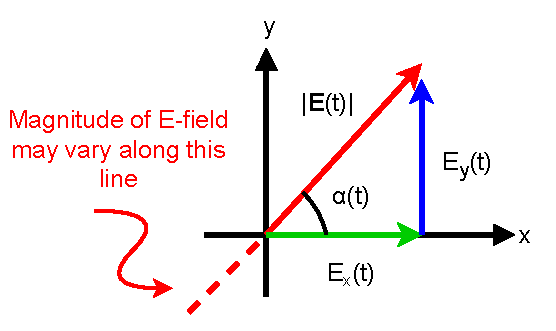
\includegraphics[width=0.6\linewidth]{images/Plane Wave Propagation/LinearPolarization.pdf}
    \caption{Linear polarization. The magnitude of the E-field may oscillate along the solid/dashed red line.}
    \label{fig:LinearPolarization}
\end{figure}

% Example 
\begin{example}
    The electric field of a plane wave is given by 
    $$ \vec{E}(z,t) = \uvec{x}\ 3\cos(\omega t - kz) + \uvec{y}\ 4\cos(\omega t - kz) $$
    Determine the (a) polarization state, (b) modulus of $\vec{E}$, and (c) orientation angle $\alpha$

    \vspace{0.25cm}
    \textbf{Solution:} 
    \begin{enumerate}[label=(\alph*)]
        \item The phase of the $x$ and $y$ components are zero ($\phi_x = \phi_y = 0$) and the phase difference is thus $\delta_s = 0$. Therefore, this plane wave is linearly polarized (LP).  

        \item The modulus $|\vec{E}|$ is 
        \begin{align*}
            |\vec{E}| &= \sqrt{E_x^2 + E_y^2} \\ 
            &= \sqrt{[3\cos(\omega t - kz)]^2 + [4\cos(\omega t - kz)]^2} \\ 
            &= \cos(\omega t - kz) \sqrt{9 + 16} \\ 
            &= 5 \cos(\omega t - kz) \qquad [\text{V/m}]
        \end{align*}

        \item The orientation angle is 
        \begin{align*}
            \alpha &= \arctan\left(\dfrac{E_y}{E_x}\right) = \arctan\left(\dfrac{4\cos(\omega t - kz)}{3\cos(\omega t - kz)} \right) = \arctan\left(\dfrac{4}{3} \right) \\ 
            &= 53.1\degree
        \end{align*}
    \end{enumerate}
\end{example}

% --- Circular Polarization 
\subsection{Circular Polarization}
For circular polarization, the magnitudes of the field components are equal ($a_x = a_y$) and the phase difference is $\delta = \pm\pi/2$. When $\delta=\pi/2$, it is called \coltextit{left-hand circular} polarization (LHCP) and when $\delta = -\pi/2$, it is called \coltextit{right-hand circular} polarization (RHCP). With LHCP, $\alpha(t)$ rotates CW, and with RHCP, $\alpha(t)$ rotates CCW with time. \par 

For both LHCP and RHCP, let's set the constants to the same value: $a_x = a_y = a$. One component will have a term with $\cos(\omega t)$ while the other will have a term with $\cos(\omega t \pm \pi/2) = \mp \sin(\omega t)$. For both cases, the magnitude turns out to be $a$: 
\begin{align}
    |\vec{E}(t)| = \sqrt{E_x^2(t) + E_y^2(t)} = \sqrt{a^2\cos^2(\omega t) + a^2\sin^2(\omega t)} = a 
\end{align}

\underline{\large \textsl{LHCP}} \\[0.25cm] 
In this case, $E_x(t) = a\cos(\omega t)$ and $E_y(t) = -a\sin(\omega t)$. The orientation over time comes out to be 
\begin{equation}
    \alpha(t) = \arctan\left(\dfrac{E_y(t)}{E_x(t)}\right) = \arctan\left(\dfrac{-a\sin(\omega t)}{a\cos\omega t} \right) = -\omega t
\end{equation}

\vspace{0.5cm}

\underline{\large \textsl{RHCP}} \\[0.25cm] 
Now, $E_x(t) = a\cos(\omega t)$ and $E_y(t) = a\sin(\omega t)$. The orientation is 
\begin{equation}
    \alpha(t) = \omega t
\end{equation}

\begin{figure}[!htp]
    \centering
    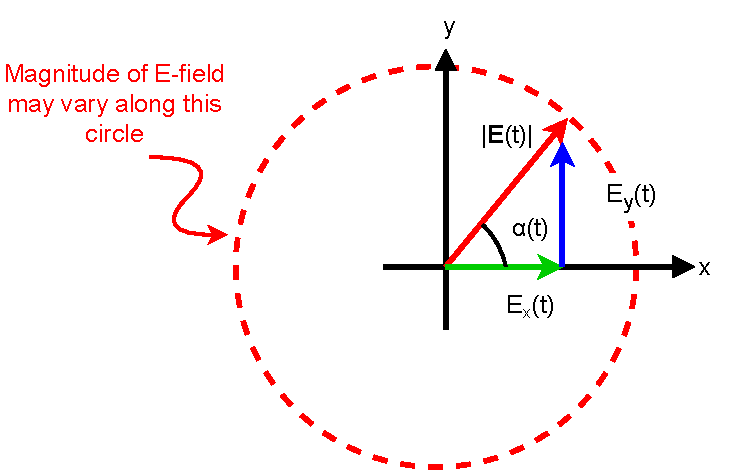
\includegraphics[width=0.7\linewidth]{images/Plane Wave Propagation/CircularPolarization.pdf}
    \caption{Circular polarization. The magnitude of the E-field may vary over the dashed circular path. If LHCP, then the vector rotates CW. If RHCP, then CCW.}
    \label{fig:CircularPolarization}
\end{figure}

% --- Elliptical Polarization 
\subsection{Elliptical Polarization}
If a wave is not linearly or circularly polarized, it is elliptically polarized. If $\delta < 0$, we have right-hand elliptical polarization, and if $\delta > 0$, it is left-hand. 

\begin{example}
    Determine the polarization state of a plane wave with electric field 
    $$ \vec{E}(z,t) = \uvec{x}\ 3\cos(\omega t - kz + 30\degree) - \uvec{y}\ 4\sin(\omega t - kz + 45\degree) $$ 

    \vspace{0.25cm}
    \textbf{Solution:} First, convert the second term to a cosine function so that it matches the first term and we can easily examine the phase difference. 
    \begin{align*}
        \vec{E} &= \uvec{x}\ 3\cos(\omega t - kz + 30\degree) - \uvec{y}\ 4\cos(\omega t - kz + 45\degree - 90\degree) \\ 
        &= \uvec{x}\ 3\cos(\omega t - kz + 30\degree) - \uvec{y}\ 4\cos(\omega t - kz - 45\degree) \\ 
        \intertext{Notice the $-\uvec{y}$. We turn this into a $+\uvec{y}$ and add 180$\degree$ of phase. }
        &= \uvec{x}\ 3\cos(\omega t - kz + 30\degree) + \uvec{y}\ 4\cos(\omega t - kz - 45\degree + 180\degree) \\ 
        &= \uvec{x}\ 3\cos(\omega t - kz + 30\degree) + \uvec{y}\ 4\cos(\omega t - kz + 135 \degree)
    \end{align*}
    We see there is a phase difference of $\delta = 135\degree - 30\degree = 105\degree$. Clearly the wave is not LP (because $\delta \neq 0$ or $180\degree$) and not CP (because $\delta \neq \pm 90\degree$). Therefore, this electric field is elliptically polarized, specifically left-handed because $\delta > 0$. 
\end{example}

% ===========================================
% Plane-Wave Propagation in Lossy Media
% ===========================================
\section{Plane-Wave Propagation in Lossy Media}

Recall the propagation constant is defined as
\begin{align}
    \gamma^2 &= -\omega^2\mu\varepsilon_c = -\omega^2\mu(\varepsilon'-j\varepsilon'') \\ 
    \gamma &= \alpha + j\beta 
\end{align}
By solving for $\alpha$ and $\beta$ by substituting these equations into the wave equation (\ref{eq:PlaneWave_WaveEqn1}), we obtain 
\begin{subequations}
\begin{empheq}[box=\eqnGreenBox]{align}
    \alpha &= \omega \left[ \dfrac{\mu\varepsilon'}{2} \left[ \sqrt{1 + \left(\dfrac{\varepsilon''}{\varepsilon'}\right)^2} -1 \right] \right]^{1/2} \qquad [\text{Np/m}] \\ 
    \beta &= \omega \left[ \dfrac{\mu\varepsilon'}{2} \left[ \sqrt{1 + \left(\dfrac{\varepsilon''}{\varepsilon'}\right)^2} + 1 \right] \right]^{1/2} \qquad [\text{rad/m}]
\end{empheq}
\end{subequations}
The intrinsic impedance of a lossy medium is 
\begin{empheq}[box=\eqnGreenBox]{align}
    \eta_c = \sqrt{\dfrac{\mu}{\varepsilon_c}} = \sqrt{\dfrac{\mu}{\varepsilon'}} \left(1 - j\dfrac{\varepsilon''}{\varepsilon'} \right)^{-1/2} \qquad [\Omega]
\end{empheq}
The distance $\delta_s$ is called the \coltextit{skin depth} and characterizes how depp an EM wave can penetrate into a conducting medium: 
\begin{empheq}[box=\eqnGreenBox]{align}
    \delta_s &= \dfrac{1}{\alpha} 
\end{empheq}
As a wave travels through a distance $z=\delta_s$, the wave magnitude decreases by a factor $e^{-1} \approx 0.37$. When $z=3\delta_s$, the magnitude is less than 5\% of its initial value. At $5\delta_s$, it is less than 1\%. \par 
Some key points about skin depth and its relation to good conductors:
\begin{itemize}
    \item In a perfect dielectric, $\sigma=0,\ \varepsilon''=0,\ \alpha=0$, thus $\delta_s=\infty$

    \item In a perfect conductor, $\sigma=\infty,\ \alpha=\infty$, thus $\delta_s = 0$. This means all incident EM waves are reflected. 

    \item For a lossy medium, the ratio $\varepsilon''/\varepsilon'$ that appears in the equations is very important. 

    \item When $\varepsilon''/\varepsilon' \ll 1$, the medium is considered to be a low-loss dielectric. 

    \item When $\varepsilon''/\varepsilon' \gg 1$, the medium is considered a good conductor. 

    \item $\varepsilon''/\varepsilon' = \sigma/(\omega\varepsilon_r\varepsilon_0)$
\end{itemize}

In a good conductor, we may approximate equations for $\alpha,\ \beta,$ and $\eta_c$ to be in a much simpler form: 
\begin{subequations}
\begin{align}
    \alpha &\approx \omega\sqrt{\dfrac{\mu\varepsilon''}{2}} = \sqrt{\pi f\mu\sigma} \\ 
    \beta &= \alpha \approx \sqrt{\pi f \mu\sigma} \\ 
    \eta_c &\approx \sqrt{j\dfrac{\mu}{\varepsilon''}} = (1+j)\sqrt{\dfrac{\pi f\mu}{\sigma}} = (1+j) \dfrac{\alpha}{\sigma}
\end{align}
\end{subequations}

\begin{example}
    A plane wave is travelling in sea water in the $+z$ direction. The constitutive parameters of sea water are $\varepsilon_r=80$, $\mu_r=1$, and $\sigma=4$ S/m. At $z=0$, the electric field is 
    \begin{align*}
        \vec{E}(t) = \uvec{x} 100\cos(10^7 \pi t)
    \end{align*}
    \begin{enumerate}[label=(\alph*), itemsep=0pt]
        \item Determine $\alpha,\ \beta,\ \eta_c,\ v_p,\ \lambda_n$ and $\delta_s$. 
        \item Find the distance at which the amplitude of the E-field is 1\% of its value at $z=0$. 
        \item Write the expressions for $\vec{E}$ and $\vec{H}$ at $z=0.8$ m as a function of time. 
    \end{enumerate}
    \textbf{Solution.} 
    \begin{enumerate}[label=(\alph*), itemsep=0pt]
        \item The angular frequency is $10^7 \pi$. Then, 
            \begin{align*}
                \dfrac{\varepsilon''}{\varepsilon'} &= \dfrac{\sigma}{\omega\varepsilon_r\varepsilon_0} = \dfrac{4}{10^7\pi \times 80 \times 8.85\times10^{-12}} \approx 180 \gg 1 
            \end{align*}
            So, sea water is a good conductor at this frequency. We may use the approximation for a good conductor with the frequency being $f=\omega/2\pi = 5$ MHz. 
            \begin{align*}
                \alpha &= \sqrt{\pi f \mu \sigma} = \sqrt{\pi \cdot (5\times10^6) \cdot (1\times 4\pi\times10^{-7}) \cdot 4} = 8.89 \text{ Np/m} \\ 
                \beta &= \alpha = 8.89 \text{ rad/m} \\ 
                \eta_c &= (1+j)\dfrac{\alpha}{\sigma} = (1+j) \dfrac{8.89}{4} = 2.22(1+j) = 2.22 e^{j\pi/4} \ \Omega \\ 
                \lambda_n &= \dfrac{2\pi}{k} = \dfrac{2\pi}{\beta} = 0.71 \ \text{m}  \\ 
                v_p &= \dfrac{\omega}{k} = \dfrac{\omega}{\beta} = \dfrac{10^7 \pi}{8.89} = 3.53 \times 10^{6} \ \text{m/s} \\ 
                \delta_s &= \dfrac{1}{\alpha} = \dfrac{1}{8.89} = 0.112\ \text{m} 
            \end{align*}

        \item The $x$-component of the electric field in lossy media takes the form 
        \begin{equation*}
            \phasor{E}_x(z) = E_{x_0} e^{-\gamma z} = \underbrace{|E_{x_0}| e^{-\alpha z}}_{\text{amplitude}} e^{-jkz}
        \end{equation*}
        where $|E_{x_0}| e^{-\alpha z}$ is the amplitude. Converting this to the time-domain, 
        \begin{equation*}
            \vec{E}(t,z) = \uvec{x}\ E_x(z) = |E_{x_0}| e^{-\alpha z} \cos(\omega t - kz)
        \end{equation*}
        At $z=0$, the amplitude is 100, which means $|E_{x_0}| e^{-\alpha \cdot 0} = |E_{x_0}| = 100$. So, we would like to find when $|E_{x_0}| e^{-\alpha z}/|E_{x_0}| = 1\% = 0.01 \implies e^{-\alpha z} = 0.01$. 
        \begin{align*}
            e^{-\alpha z} &= 0.01 \\ 
            -\alpha z &= \ln(0.01) \\ 
            z &= -\dfrac{\ln(0.01)}{\alpha} = -\dfrac{\ln(0.01)}{8.89} \\ 
            \Aboxed{z &= 0.52 \ \text{m}}
        \end{align*}

        \item At $z=0.8$ m, the amplitude is $100 e^{-(8.89)(0.8)} = 0.082$. With $k = 8.89$ rad/m, the electric field at this position is then 
        \begin{align*}
            \vec{E}(t,0.8) &= \uvec{x}\ 0.082 \cos(10^7 \pi t - 8.89 \cdot 0.8) \\ 
            &= \uvec{x}\ 0.082 \cos(10^7\pi t - 7.11\ \text{rad}) \\ 
            &= \uvec{x}\ 0.082 \cos(10^7\pi t - 47\degree) 
        \end{align*}
        In the phasor-domain, 
        \begin{equation*}
            \vecphasor{E}(0.8) = \uvec{x} \ 0.082 e^{-j 47\degree}
        \end{equation*}
        With $\eta_c = 2.22(1+j)$ and $\uvec{k}=\uvec{z}$, 
        \begin{align*}
            \vecphasor{H} &= \dfrac{1}{\eta_c} \uvec{z} \times \vecphasor{E} \\ 
            &= \dfrac{1}{2.22(1+j)} \ \uvec{y} \ 0.082 e^{-j47\degree} \\
           &= \uvec{y}\ 0.026 e^{-j92\degree}
        \end{align*}
        In the time-domain, 
        \begin{align*}
            \Aboxed{\vec{H}(t,0.8) &= \uvec{y}\ 0.026 \cos(10^7\pi t - 92\degree)}
        \end{align*}
    \end{enumerate}
\end{example} 

% ===========================================
% Current Flow in a Good Conductor
% ===========================================
\section{Current Flow in a Good Conductor}
When you connect a DC voltage across a wire, the current flowing is uniformly distributed over its cross section. That is to say, the current density $\vec{J}$ is the same along the axis of the wire and along the outer perimeter. This is not true for the ac voltage however. In the time-varying case, the current density is maximum along the perimeter and decreases exponentially as it gets closer to the axis of the wire. \par 

Consider Fig.\ \ref{fig:ExponentialDecayJ}(a) where a solid conducting block is shown. If at $z=0$ (the top planar surface), the electric field is $\vecphasor{E} = \uvec{x}\ E_0$, then the electric and magnetic field at any depth $z$ is then 
\begin{align}
    \vecphasor{E}(z) = \uvec{x}\ E_0 e^{-\alpha z} e^{-j\beta z} \\ 
    \vecphasor{H}(z) = \uvec{y}\ \dfrac{E_0}{\eta_c} e^{-\alpha z} e^{-j\beta z}
\end{align}

\begin{figure}[!htp]
    \centering
    \begin{subfigure}{0.48\linewidth}
        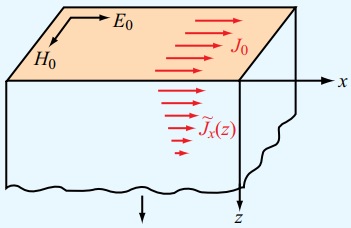
\includegraphics[width=\linewidth]{images/Plane Wave Propagation/ExponentiallyDecayingJ.png}
        \caption{Exponentially decaying $\phasor{J}_x(z)$.}
        \label{subfig:ExponentialDecayJ}
    \end{subfigure}
    \hfill
    \begin{subfigure}{0.48\linewidth}
        \centering
        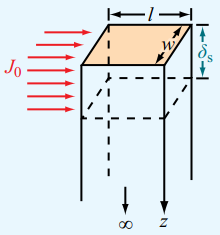
\includegraphics[width=0.6\linewidth]{images/Plane Wave Propagation/EquivalentJ0.png}
        \caption{Equivalent $J_0$ over skin depth $\delta_s$.}
        \label{subfig:EquivalentJ0}
    \end{subfigure}
    \caption{}
    \label{fig:ExponentialDecayJ}
\end{figure}

By the relation $\vec{J}=\sigma\vec{E}$, the current density is 
\begin{align}
    \vecphasor{J}(z) &= \uvec{x}\ \phasor{J}_x(z) = \uvec{x}\ \sigma E_0 e^{-\alpha z} e^{-j\beta z} = \uvec{x}\ J_0 e^{-\alpha z} e^{-j \beta z}
\end{align}
where $J_0 = \sigma E_0$. We can define the current density in terms of skin depths $\delta_s$ by using $\delta_s = 1/\alpha$ and the fact that $\alpha=\beta$ in a good conductor. 
\begin{align}
    \vecphasor{J}(z) &= \uvec{x}\ J_0 e^{-(1+j)z/\delta_s}
\end{align}
By this equation, we see clearly that the current density decays exponentially as the depth into the conductor increases. This phenomenon is called the \coltextit{skin effect}. The skin-depth influences the ac resistance. The surface impedance $Z_s$ is defined as the impedance $Z$ for a length and width $l = w = 1\ \text{m}$ and is given by 
\begin{empheq}[box=\eqnGreenBox]{equation}
    Z_s = \dfrac{1+j}{\sigma\delta_s} \qquad [\Omega]
\end{empheq}
The reactive part of $Z_s$ is positive, so $Z_s$ can be written as 
\begin{equation}
    Z_z = R_s j\omega L_s
\end{equation}
with 
\begin{align}
    R_s &= \dfrac{1}{\sigma\delta_s} = \sqrt{\dfrac{\pi f\mu}{\sigma}} \\ 
    L_s &= \dfrac{1}{\omega\sigma\delta_s} = \dfrac{1}{2} \sqrt{\dfrac{\mu}{\pi f\sigma}}
\end{align}
The ac resistance then for a slab of width $w$ and length $l$ is 
\begin{equation}
    R_\text{ac} = R_s \dfrac{l}{w} = \dfrac{1}{\sigma\delta_s w}
\end{equation}
For a coaxial cable, if $a$ and $b$ are the radii of the inner and outer conductors, respectively, the ac resistance per unit length is then 
\begin{empheq}[box=\eqnGreenBox]{equation}
    R_\text{ac, coax} = \dfrac{R_s}{2\pi} \left(\dfrac{1}{a} + \dfrac{1}{b} \right) \qquad [\Omega/\text{m}]
\end{empheq}

% ===========================================
% Power Density
% ===========================================
\section{Power Density}
The \coltextit{Poynting vector} represents the power per unit of area (power density) and is defined as 
\begin{equation}
    \vec{S} = \vec{E} \times \vec{H} \qquad [\text{W/m}^2] \label{eq:PoyntingVector}
\end{equation}
The power that flows through some surface area $A$ is then 
\begin{equation}
    P = \int\limits_A \vec{S} \cdot \uvec{n} \ dA \qquad [\text{W}]
\end{equation}
where $\uvec{n}$ is the normal unit vector to the surface. In Eq.\ (\ref{eq:PoyntingVector}), $\vec{E}$ and $\vec{H}$ are functions of time. We can express the time-averages power density $\vec{S}_\text{av}$ in terms of the fields in the phasor-domain: 
\begin{empheq}[box=\eqnGreenBox]{equation}
    \vec{S}_\text{av} = \dfrac{1}{2} \Re \{ \vecphasor{E} \times \vecphasor{H}^* \} \qquad [\text{W}/\text{m}^2]
\end{empheq}
In a \textit{lossless} medium, it can be shown that 
\begin{equation}
    \vec{S}_\text{av}(z) = \uvec{z}\ \dfrac{1}{2 \eta} (|E_{x_0}|^2 + |E_{y_0}|^2) = \uvec{z}\ \dfrac{|\vecphasor{E}|^2}{2\eta} \qquad [\text{W/m}^2]
\end{equation}
In a \textit{lossy} medium, 
\begin{equation}
    \vec{S}_\text{av}(z) = \uvec{z}\ \dfrac{|\vecphasor{E}|^2}{2|\eta_c|} e^{-2\alpha z} \cos\theta_\eta \qquad [\text{W/m}^2]
 \end{equation}
where $\eta_c = |\eta_c| e^{j\theta_\eta}$